%%%%%%%%%%%%%%%%%%%%%%%%%%%%%%%%%%%%%%%%%%%%%%%%%%%%%%%%%%%%%%%%%%%%%%%%%%%%%%%%
%2345678901234567890123456789012345678901234567890123456789012345678901234567890
%        1         2         3         4         5         6         7         8

\documentclass[letterpaper, 10 pt, conference]{ieeeconf}  % Comment this line out
                                                          % if you need a4paper
%\documentclass[a4paper, 10pt, conference]{ieeeconf}      % Use this line for a4
                                                          % paper
\usepackage{graphicx}
\IEEEoverridecommandlockouts                              % This command is only
                                                          % needed if you want to
                                                          % use the \thanks command
\overrideIEEEmargins
% See the \addtolength command later in the file to balance the column lengths
% on the last page of the document



% The following packages can be found on http:\\www.ctan.org
%\usepackage{graphics} % for pdf, bitmapped graphics files
%\usepackage{epsfig} % for postscript graphics files
%\usepackage{mathptmx} % assumes new font selection scheme installed
%\usepackage{times} % assumes new font selection scheme installed
%\usepackage{amsmath} % assumes amsmath package installed
%\usepackage{amssymb}  % assumes amsmath package installed

\title{\LARGE \bf
Comprehensive study of Communication Security in the Internet of Things (IoT) in Healthcare
}

%\author{ \parbox{3 in}{\centering Huibert Kwakernaak*
%         \thanks{*Use the $\backslash$thanks command to put information here}\\
%         Faculty of Electrical Engineering, Mathematics and Computer Science\\
%         University of Twente\\
%         7500 AE Enschede, The Netherlands\\
%         {\tt\small h.kwakernaak@autsubmit.com}}
%         \hspace*{ 0.5 in}
%         \parbox{3 in}{ \centering Pradeep Misra**
%         \thanks{**The footnote marks may be inserted manually}\\
%        Department of Electrical Engineering \\
%         Wright State University\\
%         Dayton, OH 45435, USA\\
%         {\tt\small pmisra@cs.wright.edu}}
%}

\author{Nikhil Lohia, Arizona State University\\nlohia1@asu.edu, 1211168085}


\begin{document}



\maketitle
\thispagestyle{empty}
\pagestyle{empty}


%%%%%%%%%%%%%%%%%%%%%%%%%%%%%%%%%%%%%%%%%%%%%%%%%%%%%%%%%%%%%%%%%%%%%%%%%%%%%%%%
\begin{abstract}

The advent of IoT is changing the face of health-care in a number of ways. IoT has the potential to revolutionize the way doctors interact with the patients within a health-care ecosystem. Like every upcoming technology, the security aspects of IoT health-care architecture seems to raise eyebrows and limit its applications. The recent attacks impose a question if the technology can be further carried out or not. Health-care can become a sensitive area unlike a cyber threat as the actual lives of patients is under threat. Among the communication security in Application Layer, Network Layer and Physical Layer, this report focuses on my contribution towards identifying the security issues, solution and challenges in Application Layer.
\end{abstract}


%%%%%%%%%%%%%%%%%%%%%%%%%%%%%%%%%%%%%%%%%%%%%%%%%%%%%%%%%%%%%%%%%%%%%%%%%%%%%%%%
\section{Introduction}

In the twenty first century technology has made its way into every aspect of an individual's life. From personal life to convenience, we are relying on technology and devices for our day to day tasks. An important aspect about these devices is that they are all connected to each other. Health-care is another one of those domains which is becoming technology-dependent with every upcoming advancement and innovation. From devices that measure the heart-beat of a patient, steps of an individual to devices that handle and store large amount of data all are quickly becoming a backbone of the industry.\\

\indent Health-care data is sensitive than an ordinary data. If there is a threat or attack on a car insurance data, there can only be a monetary loss. However, if we take for instance a diabetic patient whose insulin levels are controlled by a digital device, a hack into the system can threaten the life on the individual. With more and more devices coming into the picture, the security concerns are rising day by day. The concept of IoT lies on the fact that the devices are talking to each other at all times. This increases the convenience but also increases the security concerns. Thus, there comes an urgent need to regulate and safeguard such technologies in today's world. Another concern could be the large number of vendors trying to capture the market, but that is out of scope of this report. \\

\indent To understand the concerns the project investigates upon the communication security in Application Layer, Network Layer and Physical Layer. For each of the layer, we identify the security issues being addressed, findings and researches, the proposed solution and the security challenges that are encountered. Motivated by these factors I researched and explored upon the Application Layer and ways how communication can be secured in it.

\section{System Goals and Scope}
All health-care devices should communicate with each other in a fast and a secure manner. To ensure that patients and doctors receive the correct information at the right time, we need to ensure 3 major factors.
\\
\begin{itemize}
\item \textbf{Data Availability:} We need to ensure that health-related data is available and accessible by doctors and patients on-demand. This is critical to lives of individuals and can often be a major deciding factor to make surgical decisions. Patient data could be continuously transmitted over the time and thus, we need to make sure that accurate and updated information is available to the individuals in the health-care ecosystem.
\\
\item \textbf{Data Integrity:} Accurate patient information at all times is one of the major security requirements in a health-care ecosystem. This poses a major challenge to the IoT architecture as the devices are connected to each other. A hacker who gains access to confidential patient information could modify it which may lead to catastrophic consequences. This information could even be used to manipulate a patient.
\\
\item \textbf{Data encryption:} Data encryption in any kind of communication is an important aspect of security. We do not want any eavesdropping on the data by any attacker or any third party. This could result in a leak of personal and confidential information. Many encryption algorithms are used in practice for multiple applications.
\end{itemize}

\section{System Overview}
A question arises, how does the network architecture of IoT health-care ensure network security across the entire communication channel. A quick glance at all the three layers can be given as
\subsection{Application Layer}
\begin{itemize}
\item Application layer vulnerabilities
\item Solutions to address the vulnerabilities
\item Encryption algorithms at application layer
\item Sharing and presenting health-related data to the patient.
\item Offloading data from software and hardware devices and storing on servers.
\item Authorizing subjects to access patient related information.
\end{itemize}
\subsection{Network Layer}
\begin{itemize}
\item Authentication
\item Authorization
\item Encryption protocols
\item eHealth Architecture
\item Delegated authorization
\item Network security protocol
\end{itemize}
\subsection{Physical Layer}
\begin{itemize}
\item Authentication in RFID Tagging
\item DoS attack in wireless sensor networks
\item Authentication in body sensor networks
\item Security issues in wireless sensor networks
\item Cancellation based friendly jamming
\item Secure links for end-to-end communication
\end{itemize}
For the scope of this report I will concentrate on the Application Layer and the measures adopted to ensure a secure communication.

\section{Individual Contribution}
The Application Layer deals with the high-level functions of programs that may utilize the network. User interface and primary function live at this layer. Doctors access and keep track of patient information using iPads/Tablets/PDAs and all hospitals these days have monitors that display patient queue information.\\
Suppose that we apply good security through the underlying layers (1 and 2 layer), with physical isolation (layer 1), private VLANs (layer 2), and firewalls with tight packet filter policies (layers 2 and 3). But then we are deficient on our application layer security (layer seven, and often layers six and five), using un-patched server software and poorly written application and script code.

\subsection{\textbf{Hybrid security techniques for Internet of Thing Healthcare Applications}\cite{three}}
\noindent \textbf{Security Topic Addressed:} Data Encryption over communication\\
\textbf{Security Issue:} Data compromise during transmission\\
\textbf{Proposed Solution:} 
Applications need to communicate with each other using standard security techniques for the protection and immunization of databases in IoT. We cannot have a standard cryptographic technique for every communicating device in IoT healthcare. The paper suggests a hybrid cryptographic technique which is based upon the following factors
\begin{itemize}
\item Use multiple ciphers of different types to take benefit of the strength of each type of cryptography.
\item Generate a random secret key for a symmetric cipher, and then then encrypt this key via an asymmetric cipher using the recipient's public key. The recipient decrypts the secret key first and then uses that to decrypt the message.
\end{itemize}
We have 3 types of cryptographic techniques:
\begin{itemize}
\item \textbf{Secret Key Cryptography:}This technique uses the same key for both encryption and decryption.
\item \textbf{Public Key Cryptography:}This technique employs a pair of keys. One to encrypt the message and the other to decrypt the message. The advantage of this method is that the public key can be advertised by the owner to anyone who wants it.
\item \textbf{Hash Functions:}A hash function creates a fixed size blocks of data by using entry data with variable length. If the data is modified in any way, then the hash function generated will be different. This kind of security measure ensures that the information is transmitted and received exactly the way it was supposed to be. The most common hash algorithms used today are Message Digest (MD) and Secure Hash Algorithm(SHA).
\end{itemize}
\begin{figure}[!ht]
\centering
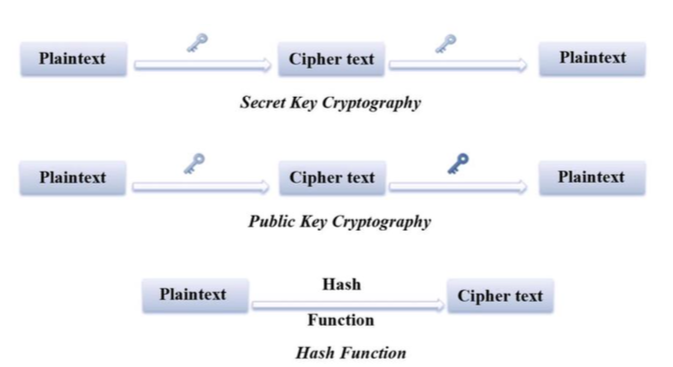
\includegraphics[width= 8.5cm]{fig1.png}
\caption{Cryptographic Methods}
\end{figure}
A Hybrid technique has combined benefits and reduce the weakness of one method as much as possible by taking the advantage of one over the other. This can be applied to several health-care applications for remote monitoring, physical activity monitoring for aging people, chronic disease management etc.\\
\textbf{Security Challenges:}
\begin{itemize}
\item Extensive use of multiple complex cryptographic functions can make the implementation cumbersome and often requires a lot of time to establish the architecture. The architecture once setup cannot be ensured that it is safe of all the attacks possible. Only with the passage of time, one can get sure enough
\item The personnel involved in setting up the architecture would be expected to know all the cryptographic techniques and a working knowledge. Replacing this personnel can have a security risk as some areas can be left exposed.
\end{itemize}

\subsection{\textbf{A Virtual PHR (Personal Health Record) Authorization System}\cite{phr}}
\noindent \textbf{Security Topic:} Policies and authorization to access patient information\\
\textbf{Security Issues:} Secure storage of patient information, maintaining the agile solution for extended periods of time\\
\textbf{Proposed Solution:} 
Any application in IoT health-care ecosystem must ensure that the individual accessing the information must be authorized to do so. One should not be allowed to access the information not intended for him. We can define a role based model for this problem, but it is also possible that an individual can have different access privileges in different environments.\\
Basically, a personal health record system consists of the following components:
\begin{itemize}
\item A non health-care component containing health and social information. Example: Information collected by family members and social networks
\item A medical device component containing health information transmitted from Internet connected medical devices. Example: Home care systems.
\item A health-care professional component containing information stored into various health-care information systems. Example: Primary care and electronic medical records
\end{itemize}
Let us take a look at the PHR authorization system proposed by the research paper.
\begin{figure}[!ht]
\centering
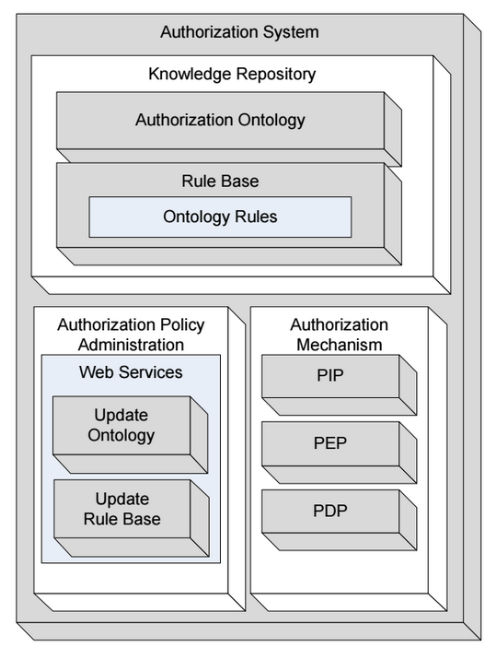
\includegraphics[width= 8.5cm]{fig2.png}
\caption{PHR Authorization System}
\end{figure}
It consists of the following components
\begin{itemize}
\item \underline{Knowledge Repository:} This repository hosts an authorization ontology and a base rule. It defines the relationships between the subjects, the environment and related attributes. It automatically infers authorization based upon the RABAC model and applies the required permissions.
\item \underline{Authorization Policy Administration:} This module uses a a bunch of web services to update the knowledge repository based upon the information collected from several devices. It basically updates the ontology and base rule.
\item \underline{Authorization Mechanism:} It consists of 3 parts
\begin{enumerate}
\item PIP (Policy Information point) creates subject to role rules
\item PEP (Policy Enforcement point) creates the subject to access requests
\item PDP (Policy Decision point) combines information from the above 2 points and makes a decision whether the access should be permitted or denied.
\end{enumerate}
\end{itemize}
\textbf{Security Challenges:} 
\begin{itemize}
\item In this cloud-based PHR environment, the system is implemented as a service which assumes that health-care system are interlaced with interacting services. This means that the authorization information and personnel roles should have the capability to be extracted on the fly.
\item One major concern is that all potential subjects are not known in advance. Such a system would require constant updates and a learning methodology to implement.
\end{itemize}

\section{Findings and Analysis}
There can be a lot of challenges when handling data in IoT devices and applications. This data if placed in wrong hands can be dangerous and reveal private information about the patient.
\begin{itemize}
\item We have several security and encryption techniques available to secure information communication between two nodes but when it comes to health-devices we cannot afford them to be expensive. One major point to consider about health-care devices is also that they should not be power hungry. We need to use techniques that takes care of memory requirements and power utilization as well.\\
The research paper\cite{three} suggests to use hybrid cryptographic techniques to ensure secure transmission of information. We can use a mixture of two such that the shortcomings of one can be traded with the benefits of other. Such techniques must however by applied with care as the architecture could become complex to manage over time.
\item Information authorization is also really important in an IoT health-care ecosystem. The fact that all devices are connected to each other can become a threat if the authorization mechanism is not put into place correctly. A ``cardiologist'' must not be able to access the information related to brain of the patient. However, a brain surgeon must have access to the heart information if he is inside the ``hospital cardiology department''. Thus, the environment also makes a difference for who can access an information.\\
The PHR system addressed in the research paper\cite{phr} defines a role and architecture based access control system which helps in determining which kind of role will be assigned to the subject.
\end{itemize}

\section{Recommendations}
Developing a system to ensure proper authorization and access control not only increases transparency but also encapsulates the information. 
\begin{itemize}
\item
Such kind of a protocol can be followed by maintaining en exhaustive hierarchy of user roles and their working environment. This is essential because different settings could change a user role. A personnel can have different access rights under different circumstances as well. An emergency situation could call for an information required which is generally not available for an individual. Hence, rules must be made keeping all such situations in mind.
\item Sharing information between applications should take advantage of hybrid cryptographic methods. The weakness of a method must be identified and a stronger method must not be implemented just because it is available. The applications in an IoT health-care ecosystem require only specific controls and the encryption standards must be evaluated before implementing them.
\end{itemize}

\section{Conclusion}

IoT as a new technology has been more widely used and is constantly evolving. Even in health-care applications; the open nature of the information/data media has brought risks to the security of the wireless sensor networks and their collected data. Several techniques can be applied in securing the data transmission between these applications but we need to make sure that it remains cheap and efficient. Apart from the transmission we also need a system on the application level to determine which user can access which information. There cannot be an exhaustive set of rules to determine which subject has what role. A system needs to be created in such a way that the subjects are assigned roles dynamically based upon the environment they are
working in.\\
\indent Many people around the world have access to some kind of PHR but problems regarding privacy and security of patient sensitive data could pose a serious impediment to further PHR development and usage. The main objective of the authorization system is to empower patient control to their health and social data and enable providers to share their data with others in order to support continuity of care.

\begin{thebibliography}{99}

\bibitem{one} Al-Janabi, Samaher, et al. ``Survey of main challenges (security and privacy) in wireless body area networks for healthcare applications.'' \emph{Egyptian Informatics Journal}, (2016).

\bibitem{phr} Poulymenopoulou, Mikaela, Flora Malamateniou, and George Vassilacopoulos. ``A virtual PHR authorization system.'' \emph{Biomedical and Health Informatics (BHI)}, 2014 IEEE-EMBS International Conference on. IEEE, 2014.

\bibitem{three} Yehia, Lobna, Ayman Khedr, and Ashraf Darwish. ``Hybrid Security Techniques for Internet of Things Healthcare Applications.'' \emph{Advances in Internet of Things}, 5.03 (2015): 21.d

\bibitem{four} Gong, Tianhe, et al. ``A medical healthcare system for privacy protection based on IoT.'' \emph{Parallel Architectures, Algorithms and Programming (PAAP)}, 2015 Seventh International Symposium on. IEEE, 2015.


\end{thebibliography}




\end{document}
